% SPAR Fall 2026 midterm report, due Monday 2 November 2026 (Anywhere on Earth).
% SPAR asks for 500 to 1,000 words. Word targets per section follow the SPAR
% empirical outline. Keep the abstract as plain text: it is pasted into the
% submission form.
%
% Updated 20 Oct (Nat): simulation results from runs 3-5, four figures, a plan
% for the second half. Figures come from the simulation repo (results/fifth_run)
% and figures/make_*.py; rebuild them there rather than editing the PDFs.
% Items marked TODO need a check before submission.
\documentclass[11pt,a4paper]{article}

\usepackage[T1]{fontenc}
\usepackage[utf8]{inputenc}
\usepackage{lmodern}
\usepackage[margin=2.5cm]{geometry}
\usepackage{booktabs}
\usepackage{array}
\usepackage{parskip}
\usepackage{graphicx}
\usepackage{float}
\usepackage{tikz}
\usetikzlibrary{arrows.meta,positioning,calc}
\usepackage[font=small,labelfont=bf]{caption}
\usepackage[hidelinks]{hyperref}

\title{Verification Evidence for Compute Governance:\\What Inspection Regimes Actually Detect}
% Author order to be agreed by the team before submission.
\author{Sidar Aslanoglu \and Vir Khosla \and Joon Baek \and Max Perin \and Nat Elder \and Jonas Kgomo \and Joel Naoki Christoph\\[0.6em]
\small SPAR Fall 2026}
\date{}

\begin{document}
\maketitle

\begin{abstract}
% 45 to 90 words. Write last. No citations.
Proposals to verify agreements on frontier AI compute assume that their instruments detect violations. We test that assumption. For each instrument, we code the evidence on its measured performance and pair it with an analogue from a regime that has run in practice. Of four coded instruments, two have a measured catch rate, both from laboratory tests. A compliance model shows that the inputs that decide whether cheating pays, the size of fines and the cheapest way to evade, are the least measured.
\end{abstract}

\section{Introduction}
% 90 to 175 words.
Compute governance proposals rely on a small set of verification instruments: satellite imagery of data centres, on-chip attestation, compute metering, third-party verifiers and others. The proposals state what each instrument should detect. Few report how often it does, at what false-alarm rate or under what evasion. Without these numbers, policymakers cannot tell whether an inspection regime would deter a developer from under-reporting compute.

Our research question is what the existing evidence shows about the detection performance of compute verification instruments. We code that evidence directly where it exists. Where it does not, we turn to analogues from inspection regimes with a track record. We then feed the coded values into a compliance model to find the fine at which honest reporting pays, and which missing numbers that answer depends on most.

\section{Related work}
% 65 to 130 words. Three to five closest works.
Shavit \cite{shavit2023} proposes compute monitoring through on-chip firmware and sets design targets for detecting large training runs. Aarne, Fist and Withers \cite{aarne2024} describe on-chip mechanisms such as remote attestation. Wasil et al.\ \cite{wasil2024} survey verification methods for international AI agreements. Baker \cite{baker2023} draws lessons for AI treaties from nuclear arms control verification. Christoph \cite{christoph2026} models compute permit markets under imperfect monitoring; our simulation extends that model, following Kaplow and Shavell \cite{kaplow1994}. These works propose instruments or draw analogies. None of them collects measured detection performance across instruments. % TODO: confirm for Wasil et al.

\section{Methods}
% 110 to 200 words.
We keep a case register of instruments from published proposals. An instrument enters the register if it passes four tests. It appears in a published compute governance proposal. It is one instrument: one object checked by one kind of observation, able to raise an alarm on its own. It does not duplicate an existing row under another name. It verifies a claim; restrictions such as export controls are out.

For each instrument, a coder fills a row with the object verified, the method, the access needed, the threat model and any measured performance, with page references. The coder pairs it with analogues from other regimes and records the published target, measured results, inspection effort and known evasion. Two labels go with every pair: evidence confidence and transfer confidence. Each instrument is assigned two independent coders. A final field tags which model input the row informs (Figure~\ref{fig:pipeline}).

Each tagged value becomes a range, marked as measured, stand-in or guess. In the model a developer hides compute when the saving exceeds the expected penalty: checking rate times catch rate times the chance of punishment times the fine \cite{christoph2026,kaplow1994}. When several instruments run together, the developer picks the one route past them that pays best. Each result draws 2,000 sets of inputs \cite{simrepo}.

\begin{figure}[t]
\centering
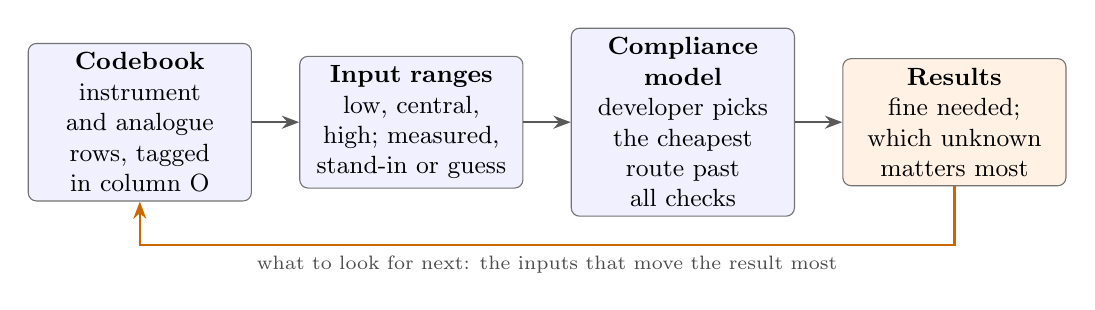
\begin{tikzpicture}[
  box/.style={draw=black!55, rounded corners=3pt, align=center, font=\small, minimum height=1.25cm, text width=2.6cm, fill=#1},
  box/.default=white,
  arr/.style={-{Stealth[length=2.2mm]}, thick, draw=black!65},
  lab/.style={font=\scriptsize, text=black!70, align=center}]
\node[box=blue!6] (code) {\textbf{Codebook}\\instrument and analogue rows, tagged in column O};
\node[box=blue!6, right=0.6cm of code] (range) {\textbf{Input ranges}\\low, central, high; measured, stand-in or guess};
\node[box=blue!6, right=0.6cm of range] (model) {\textbf{Compliance model}\\developer picks the cheapest route past all checks};
\node[box=orange!10, right=0.6cm of model] (out) {\textbf{Results}\\fine needed; which unknown matters most};
\draw[arr] (code) -- (range);
\draw[arr] (range) -- (model);
\draw[arr] (model) -- (out);
\draw[arr, draw=orange!80!black] (out.south) -- ++(0,-0.75) -| node[lab, pos=0.25, below] {what to look for next: the inputs that move the result most} (code.south);
\end{tikzpicture}
\caption{How evidence reaches the model and how the model directs the next round of coding.}
\label{fig:pipeline}
\end{figure}

\section{Results}
% 155 to 265 words.
\subsection{Evidence}
Table~\ref{tab:rows} shows the first coded rows: four instruments, each paired with one analogue. Figure~\ref{fig:evidence} maps what backs each model input.

\begin{table}[h]
\centering
\footnotesize
\begin{tabular}{@{}llp{3.3cm}l@{}}
\toprule
Instrument & Analogue & Measured catch rate & Evidence\textsuperscript{a} \\
\midrule
CI-02 Third-party verifiers & EU emissions trading & none & high \\
CI-03 On-chip attestation & IAEA remote monitoring & none & high \\
CI-04 Compute metering & Nuclear material accountancy & lab 98\%; 43\% against best evasion & high \\
CI-05 Satellite imagery & IAEA satellite imagery & lab 98.6\%, unhidden sites only & medium \\
\bottomrule
\end{tabular}
\caption{First coded rows, one coder per row. Each line is one instrument row and its analogue row. CI-01 (cloud reporting) has no coder yet.\\
\textsuperscript{a} Evidence confidence covers the coded findings as a whole, not a catch rate.}
\label{tab:rows}
\end{table}

Two instruments have a measured catch rate, both from laboratory tests. A classifier found 98.6\% of data centres in 230 images, with every miss below 4\,MW \cite{clymer}; its tests did not include concealment. GPU telemetry detected 98\% of training runs, but only 43\% when the evader knew how the detector worked \cite{rahman2026}. None of the four analogues reports a catch rate. Two inputs have no evidence for any instrument: how large fines are relative to the gain from cheating, and how often detection leads to a penalty.

\begin{figure}[t]
\centering
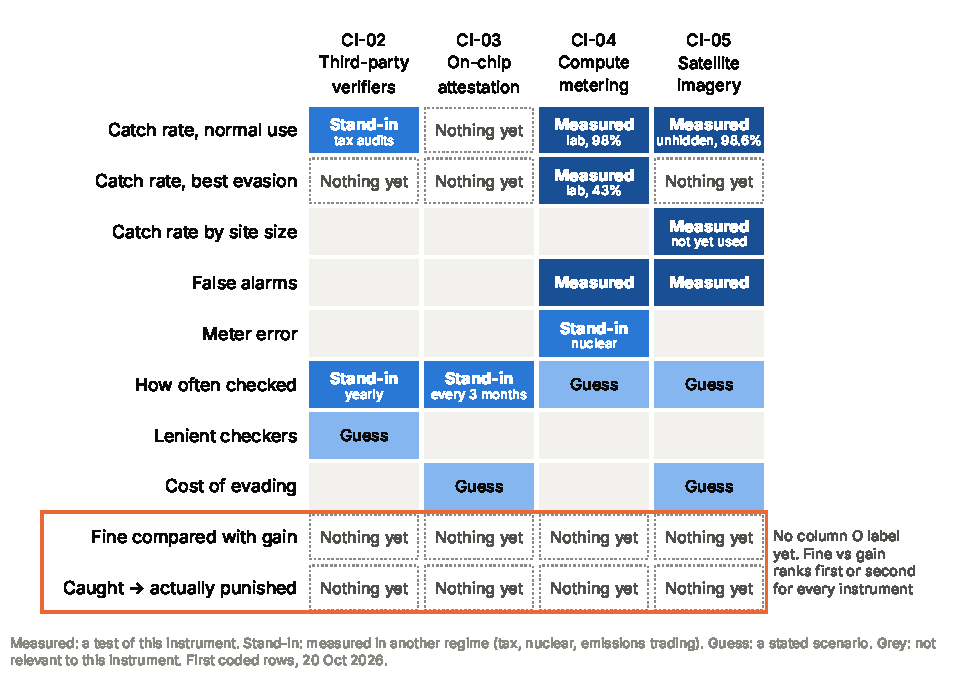
\includegraphics[width=\linewidth]{figures/evidence_map.pdf}
\caption{What backs each model input, by instrument. The two boxed rows have no evidence anywhere and no label in the codebook yet.}
\label{fig:evidence}
\end{figure}

\subsection{Simulation}
Results use placeholder ranges wherever evidence is missing, so they show which numbers matter, not what the true values are.

\emph{The fine, not the checking rate, is the question.} Most instruments already check about once a year. At that rate, a fine of 2--3 times the gain deters a developer facing an honest checker. A lenient verifier raises this to about 10 times.

\emph{Multiplying catch rates overstates a regime.} A cheater does not face each check in turn: it picks one route past all of them. With route choice, the fine needed is 2.0 times the gain with middle-range inputs and 4.4 times in a worst case; multiplying the same catch rates gives 1.1 and 1.4 (Figure~\ref{fig:regime}). Cheaters almost never go past the meter. They defeat attestation, or use a hidden site, so satellites carry the regime: without them the fine needed rises to about 14 times.

\emph{Small, slow runs are the hard ones.} A 10\textsuperscript{26} FLOP run takes about a month on 100,000 GPUs or 2.7 years on 3,000 GPUs in small sites that imagery mostly misses. The fine needed rises from about 2 times for the first to 7--10 times for the second (Figure~\ref{fig:size}).

\begin{figure}[t]
\centering
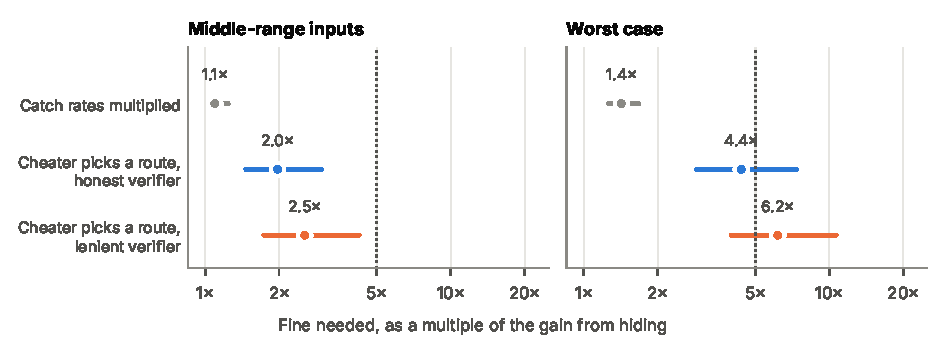
\includegraphics[width=\linewidth]{figures/regime.pdf}
\caption{Fine needed for a regime of verifiers, attested metering and satellite imagery. Dot: median over 2,000 draws; line: 10th--90th percentile; dotted line: the main assumption of a fine 5 times the gain.}
\label{fig:regime}
\end{figure}

\begin{figure}[t]
\centering
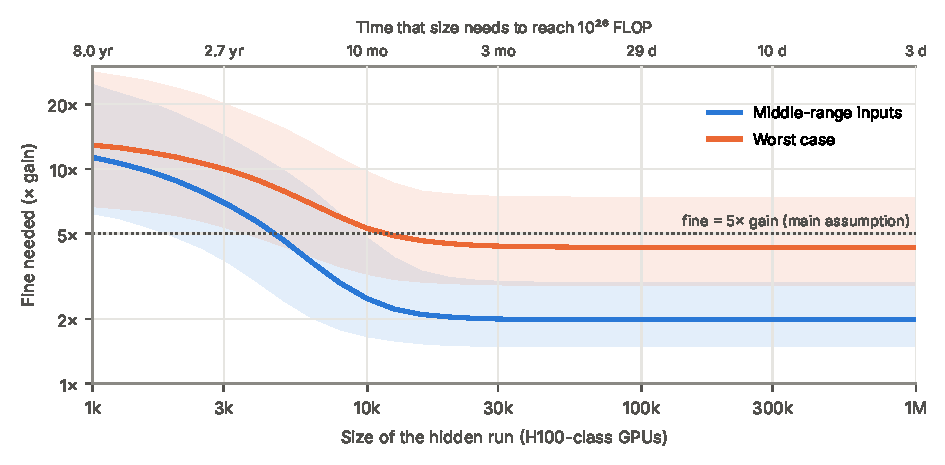
\includegraphics[width=\linewidth]{figures/size.pdf}
\caption{Fine needed against the size of a hidden run. The cheater splits the run across as many sites as suits it; each extra site costs efficiency. Top axis: time that size needs to reach 10\textsuperscript{26} FLOP at 40\% utilisation.}
\label{fig:size}
\end{figure}

\section{Discussion}
% 110 to 175 words.
Proposals assume detection rates that few sources measure, and the analogues we expected to fill the gap do not report them either. The model also shows that detection is one of three inputs that decide deterrence, with the size of the fine and the chance a caught developer is punished. Neither has been coded. A measured catch rate matters only for the route a cheater would actually use: laboratory rates against cooperative subjects say little about a strategic evader. Flat caps on fines, as in California SB~53 \cite{sb53} and the New York RAISE Act \cite{raise}, fail when a few large developers dominate.

The study has three limitations so far. Each row has one coder. Most ranges are placeholders. Four instruments cover a small part of the proposals. Table~\ref{tab:plan} sets out the second half.

\begin{table}[H]
\centering
\footnotesize
\begin{tabular}{@{}lp{0.72\linewidth}@{}}
\toprule
By & Work \\
\midrule
21 Oct & Agree four new codebook tags: fine vs gain, punishment follow-through, evasion cost, worst-case catch rate \\
9 Nov & Second coder rows in; agreed worst-case values; rerun with coded ranges \\
24 Nov & Code cloud reporting (CI-01) and chip tracking, the checks that cover slow runs; replace the guessed site-size curve with coded values \\
14 Dec & Judge instruments used between states on timeliness (caught before a run finishes); final figures and summary table \\
\bottomrule
\end{tabular}
\caption{Plan for the second half.}
\label{tab:plan}
\end{table}

\section{Conclusion}
% 45 to 90 words.
Measured evidence on the detection performance of compute verification instruments is thin, and it is thinnest where it matters most: against deliberate evasion, and on the sanctions that follow detection. Our coded dataset shows this gap instrument by instrument. Our compliance model shows which missing numbers decide whether an inspection regime deters cheating, and so where the second half of the project should look.

\begin{thebibliography}{99}
\bibitem{aarne2024} O.~Aarne, T.~Fist and C.~Withers, \emph{Secure, Governable Chips: Using On-Chip Mechanisms to Manage National Security Risks from AI \& Advanced Computing}. Center for a New American Security, January 2024.
\bibitem{baker2023} M.~Baker, ``Nuclear Arms Control Verification and Lessons for AI Treaties,'' arXiv:2304.04123, 2023.
\bibitem{christoph2026} J.~N.~Christoph, ``Risk-Weighted Compute Permit Markets under Imperfect Monitoring,'' SSRN working paper 6361077, 2026.
\bibitem{clymer} J.~Clymer, ``Data centers that are not deliberately concealed will be easy to locate,'' 2025. Code: \url{https://github.com/Joshuaclymer/data_center_classifier}. % TODO: venue
\bibitem{kaplow1994} L.~Kaplow and S.~Shavell, ``Optimal Law Enforcement with Self-Reporting of Behavior,'' \emph{Journal of Political Economy} 102(3): 583--606, 1994.
\bibitem{rahman2026} Rahman and Tajdari, 2026, ICML workshop paper on detecting training runs from GPU telemetry, as coded in row CI-04. % TODO: full authors and title from Vir's row
\bibitem{raise} New York Responsible AI Safety and Education (RAISE) Act, 2025, as amended. % TODO: check the current penalty provisions after the chapter amendments
\bibitem{sb53} California Senate Bill 53, Transparency in Frontier Artificial Intelligence Act, 2025.
\bibitem{shavit2023} Y.~Shavit, ``What Does It Take to Catch a Chinchilla? Verifying Rules on Large-Scale Neural Network Training via Compute Monitoring,'' arXiv:2303.11341, 2023.
\bibitem{simrepo} N.~Elder, Verification-Evidence-Simulation, \url{https://github.com/marketshaping/Verification-Evidence-Simulation}, fifth run, 20 October 2026.
\bibitem{wasil2024} A.~R.~Wasil et al., ``Verification Methods for International AI Agreements,'' arXiv:2408.16074, 2024.
\end{thebibliography}

\end{document}
